%!TEX TS-program = xelatex
\documentclass[12pt, a4paper, oneside]{article}

\usepackage{amsmath,amsfonts,amssymb,amsthm,mathtools}  % пакеты для математики

\usepackage[utf8]{inputenc} % задание utf8 кодировки исходного tex файла
\usepackage[british,russian]{babel} % выбор языка для документа
\usepackage[X2,T2A]{fontenc}        % кодировка

\usepackage{fontspec}         % пакет для подгрузки шрифтов
\setmainfont{Helvetica}   % задаёт основной шрифт документа

% why do we need \newfontfamily:
% http://tex.stackexchange.com/questions/91507/
\newfontfamily{\cyrillicfonttt}{Helvetica}
\newfontfamily{\cyrillicfont}{Helvetica}
\newfontfamily{\cyrillicfontsf}{Helvetica}

\usepackage{unicode-math}     % пакет для установки математического шрифта
\setmathfont{Neo Euler}      % шрифт для математики
% \setmathfont[math-style=ISO]{Asana Math}
% Можно делать смену начертания с помощью разных стилей

% Конкретный символ из конкретного шрифта
% \setmathfont[range=\int]{Neo Euler}

%%%%%%%%%% Работа с картинками %%%%%%%%%
\usepackage{graphicx}                  % Для вставки рисунков
\usepackage{graphics}
\graphicspath{{images/}{pictures/}}    % можно указать папки с картинками
\usepackage{wrapfig}                   % Обтекание рисунков и таблиц текстом

%%%%%%%%%%%%%%%%%%%%%%%% Графики и рисование %%%%%%%%%%%%%%%%%%%%%%%%%%%%%%%%%
\usepackage{tikz, pgfplots}  % язык для рисования графики из latex'a

%%%%%%%%%% Гиперссылки %%%%%%%%%%
\usepackage{xcolor}              % разные цвета

\usepackage{hyperref}
\hypersetup{
	unicode=true,           % позволяет использовать юникодные символы
	colorlinks=true,       	% true - цветные ссылки, false - ссылки в рамках
	urlcolor=blue,          % цвет ссылки на url
	linkcolor=red,          % внутренние ссылки
	citecolor=green,        % на библиографию
	pdfnewwindow=true,      % при щелчке в pdf на ссылку откроется новый pdf
	breaklinks              % если ссылка не умещается в одну строку, разбивать ли ее на две части?
}


\usepackage{todonotes} % для вставки в документ заметок о том, что осталось сделать
% \todo{Здесь надо коэффициенты исправить}
% \missingfigure{Здесь будет Последний день Помпеи}
% \listoftodos --- печатает все поставленные \todo'шки

\usepackage{enumitem} % дополнительные плюшки для списков
%  например \begin{enumerate}[resume] позволяет продолжить нумерацию в новом списке

\usepackage[paper=a4paper, top=20mm, bottom=15mm,left=20mm,right=15mm]{geometry}
\usepackage{indentfirst}       % установка отступа в первом абзаце главы

\usepackage{setspace}
\setstretch{1.15}  % Межстрочный интервал
\setlength{\parskip}{4mm}   % Расстояние между абзацами
% Разные длины в латехе https://en.wikibooks.org/wiki/LaTeX/Lengths


\usepackage{xcolor} % Enabling mixing colors and color's call by 'svgnames'

\definecolor{MyColor1}{rgb}{0.2,0.4,0.6} %mix personal color
\newcommand{\textb}{\color{Black} \usefont{OT1}{lmss}{m}{n}}
\newcommand{\blue}{\color{MyColor1} \usefont{OT1}{lmss}{m}{n}}
\newcommand{\blueb}{\color{MyColor1} \usefont{OT1}{lmss}{b}{n}}
\newcommand{\red}{\color{LightCoral} \usefont{OT1}{lmss}{m}{n}}
\newcommand{\green}{\color{Turquoise} \usefont{OT1}{lmss}{m}{n}}

\usepackage{titlesec}
\usepackage{sectsty}
%%%%%%%%%%%%%%%%%%%%%%%%
%set section/subsections HEADINGS font and color
\sectionfont{\color{MyColor1}}  % sets colour of sections
\subsectionfont{\color{MyColor1}}  % sets colour of sections

%set section enumerator to arabic number (see footnotes markings alternatives)
\renewcommand\thesection{\arabic{section}.} %define sections numbering
\renewcommand\thesubsection{\thesection\arabic{subsection}} %subsec.num.

%define new section style
\newcommand{\mysection}{
	\titleformat{\section} [runin] {\usefont{OT1}{lmss}{b}{n}\color{MyColor1}} 
	{\thesection} {3pt} {} } 


%	CAPTIONS
\usepackage{caption}
\usepackage{subcaption}
%%%%%%%%%%%%%%%%%%%%%%%%
\captionsetup[figure]{labelfont={color=Turquoise}}

\usepackage[normalem]{ulem}  % для зачекивания текста

\pagestyle{empty}

\begin{document}

\section*{Задание 3 :  резюме (15 баллов)}

Когда человек хочет найти работу, он пишет резюме. Скорее всего, вы тоже рано или поздно будете искать работу.  Пришло время написать себе резюме с помощью \LaTeX{}!

Перед тем как заняться этим, прочитайте \href{https://vk.com/@thevyshka-kak-luchshe-oformit-rezume-kommentarii-hr-specialista}{небольшую заметку с вышкинского паблика} про резюме. Подумайте о том, почему $3$ из $4$ резюме, описанных в статье, не очень хорошие. 

Когда будете размышлять об этом, представляйте себя hr. Вы в течение часа должны просмотреть около 100 резюме и отобрать 10 лучших. На каждое у вас есть примерно по полминуты. 

Резюме вы можете оформить самостоятельно или воспользоваться одним из теховских шаблонов из интернетов. Вы можете сделать это как на русском, так и на английском языке. Не забудьте указать  \LaTeX{} в числе программ, которыми вы умеете пользоваться!  

Обычно, поначалу резюме получается очень пустым. Ты сидишь и пытаешься вспомнить хоть какие-то свои регалии, и ничего не лезет в голову. В итоге включается фантазия, и ты начинаешь заполнять своё CV немного преукрашенными штуками. Например, вот так один мой друг описал свой опыт работы в приёмке: 

\begin{center}
	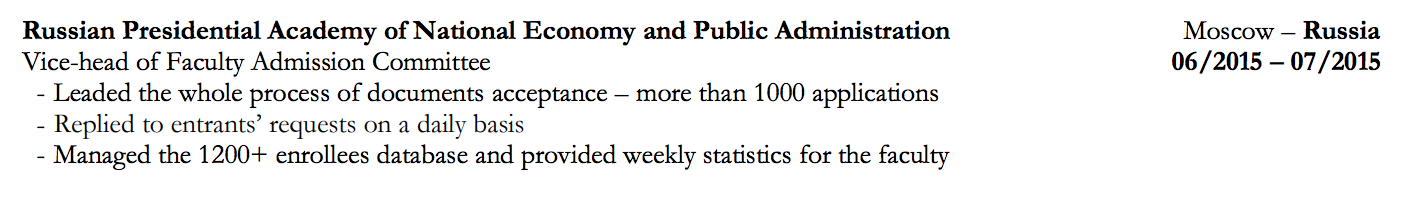
\includegraphics[scale=0.35]{sasha.png}
\end{center}

Каждый раз, когда читаю это, возникает ощущение, что он на своих плечах поднял целое министерство. По мере накопления регалий, с болью в сердце, какие-то куски из резюме придётся выкидывать. На одной странице много регалий не помещается.

\begin{itemize}
	\item[$(10)$] Вы сделали адекватное резюме.
	\item[$(5)$] Увидев ваше резюме, я захотел, чтобы вы сделали для меня кое-какую грязную работку.
\end{itemize}

Итоговый pdf-файл, tex-файл и все картинки, которые использовались в документе, нужно положить в папку на свой Dropbox, Github, yandex-disk или другой репозиторий. После нужно заполнить \href{https://docs.google.com/forms/d/e/1FAIpQLSe11kxKVfv07iCL1E9yNX7ll9swKImiVwRr1H70lslGzInRSg/viewform}{уютную гугл-форму.}  

Если вы выполняете работу в overleaf, то прикрепляйте в форму ссылку на неё. Если вы прикрепите ссылку с возможностью редактирования вашего файла, при проверке мы оставим у вас в файле полезные комментарии. Если вы кидаете ссылку на репозиторий, все комменты отправим в личку.

Перед этим обязательно проверьте компилируется ли файл без ошибок на вашем компьютере. Не стесняйтесь абсолютно в любое время дня и ночи просить о помощи, если она вам действительно необходима! \textbf{Также не забывайте про то, что любое творчество поощряется,} а ещё не забываете, где  находится  \href{https://fulyankin.github.io/LaTeX/}{страничку курса} с кучей шпаргалок!

\end{document}
